%------------------------------------------------------------------------------
%	CAPITOLO 12
%------------------------------------------------------------------------------

\chapter{Un'antica lettera amorosa}
Un vagheggino\footnote{Corteggiatore fatuo e galante} del paese pretendeva una ragazza dei \index[Personaggi]{Salvatori (famiglia)}Salvatori. Per farle giungere i palpiti del suo cuore le inviava delle lettere. Ecco la risposta definitiva della ragazza:\\ 
\indent <<Siete il più bifolco, stracio del paese, finitela>>.\footnote{Il più bifolco e straccione del paese} 

 \begin{figure}[htb]
    \centering
    %\vspace{-0.7cm}
    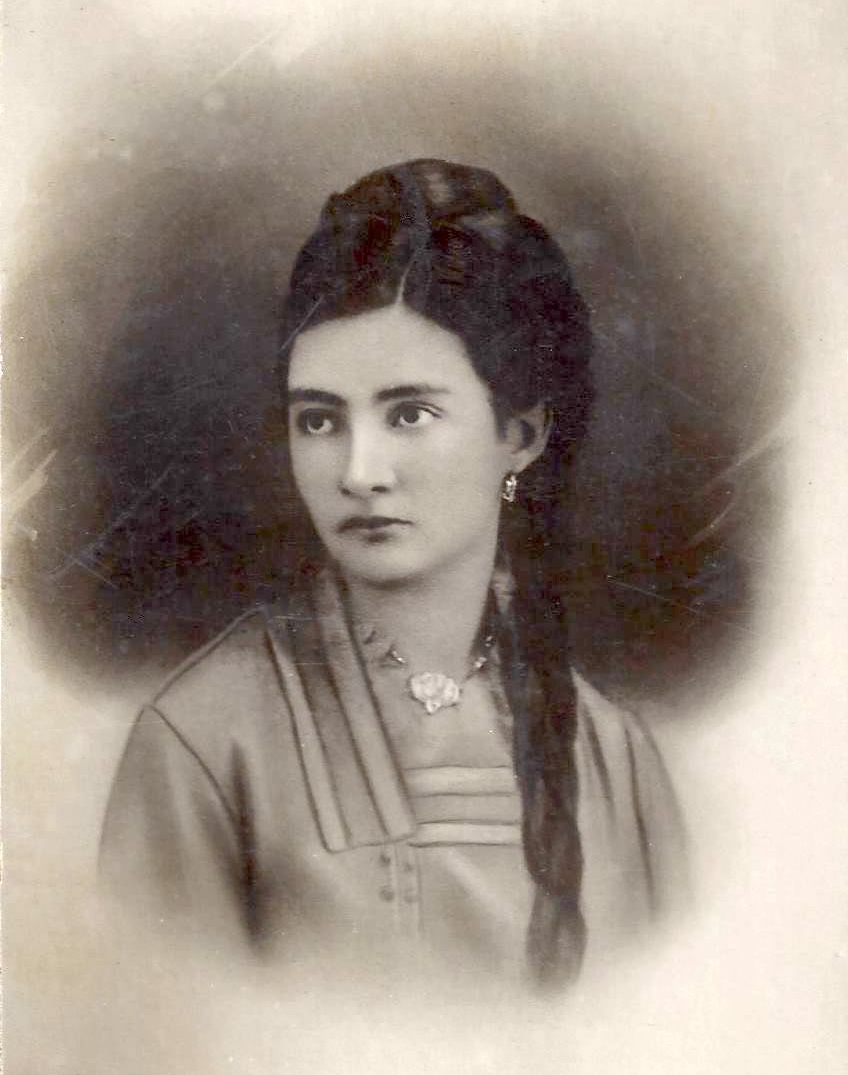
\includegraphics[width=\textwidth]{mariannina}
    \caption[Mariannina Gagliardi]{\textbf{Mariannina Gagliardi}\index[Personaggi]{Gagliardi Mariannina} (1860 - 1882), madre di Stefano. Studiò all'università di Bologna e terminati gli studi si sposò con Natale \index[Personaggi]{Mingazzi Natale}Mingazzi. Morì di tubercolosi a soli 22 anni il 23 settembre 1882 quando Stefano non aveva neanche due anni. Come era solito fare, ai nuovi nati si dava il nome di parenti morti precocemente ed infatti mia nonna prese il nome della madre di Stefano quando nacque nel 1927.  \label{fig:mariannina}}
    %\vspace{-0.3cm}
\end{figure}